% !TeX root = ../main-presentation.tex
\begin{frame}
    \frametitle{What are we going to be talking about?}
    \pause
    \centering
    \LARGE
    Digital circuits!

    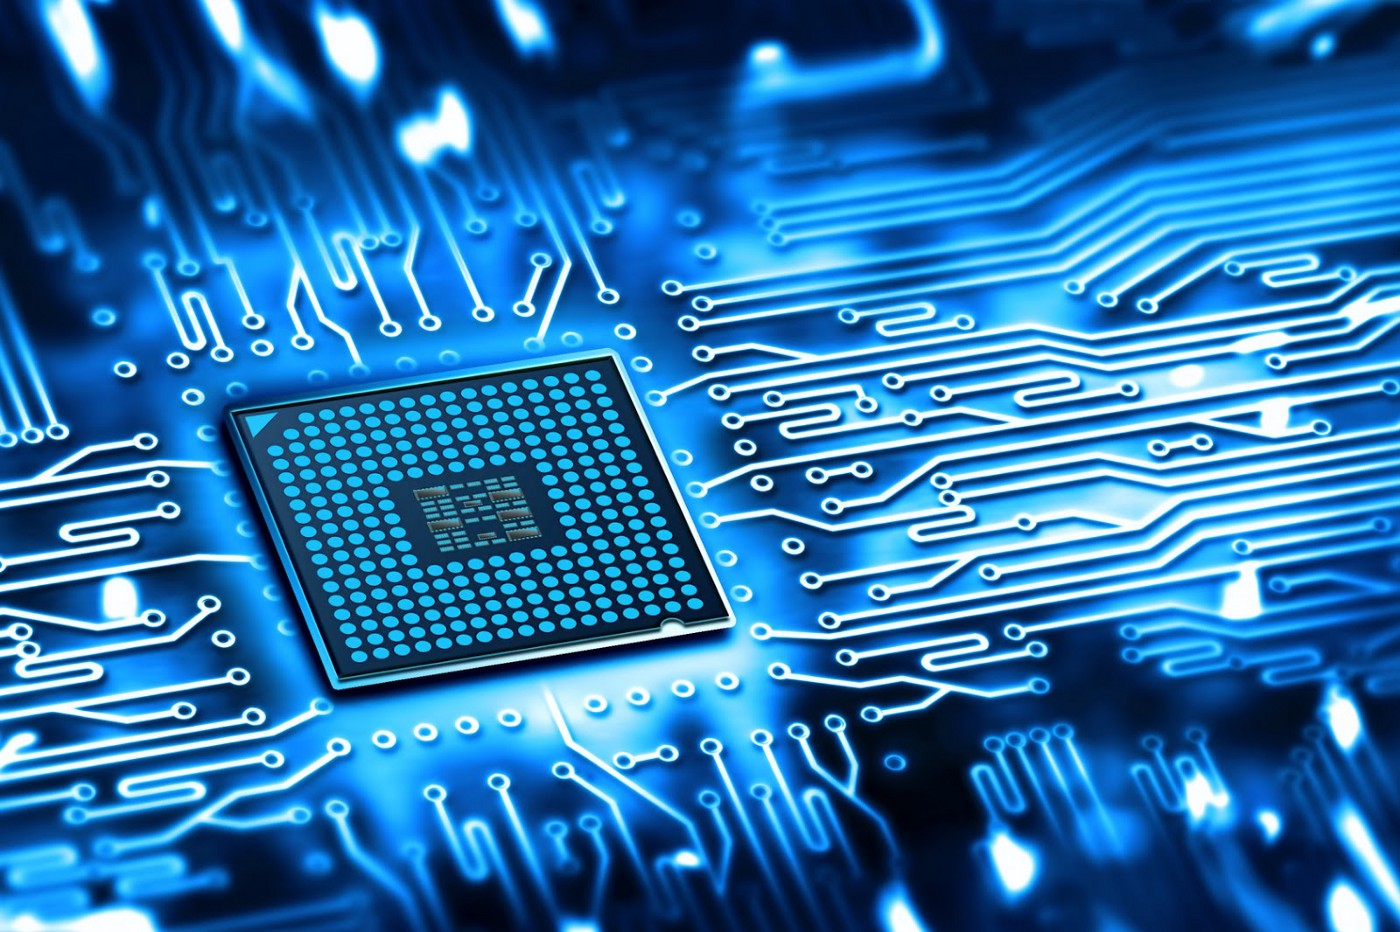
\includegraphics[width=0.6\textwidth]{imgs/circuit}
\end{frame}
\begin{frame}
    \frametitle{What are we going to be talking about?}
    \centering
    \LARGE
    Digital circuits!

    \vspace{1em}
    \normalsize

    \scalebox{2}{\tikzfig{circuits/examples/sr-latch/real-circuit}}
\end{frame}
\begin{frame}
    \frametitle{What are we going to be talking about?}

    \pause

    \centering
    \LARGE
    We want a \alert{compositional} theory of digital circuits.

    \vspace{0.5em}

    \normalsize

    \pause
    \dsptikzfig{strings/category/f}[box=F,colour=seq]
    \pause
    \quad
    \dsptikzfig{strings/category/f}[box=G,colour=seq]
    \pause
    \quad
    \dsptikzfig{strings/category/f-2-2}[box=H,colour=seq]

    \pause
    \vspace{1em}

    \dsptikzfig{strings/category/composition}[box1=F,box2=G,colour=seq]
    \quad
    \dsptikzfig{strings/monoidal/tensor}[box1=F,box2=G,colour=seq]
    \quad
    \dsptikzfig{strings/traced/trace-rhs}[box=H,colour=seq]

\end{frame}

\begin{frame}
    \frametitle{Why all the pictures?}
    \centering

    \LARGE
    We want to reason \alert{equationally} about circuits.

    \pause

    Using \alert{string diagrams} removes much of the bureacracy

\end{frame}

\begin{frame}
    \frametitle{The story so far}

    \pause
    \centering

    \scalebox{8}{\textbf{2003}}

\end{frame}

\begin{frame}
    \frametitle{The story so far}

    \centering
    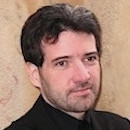
\includegraphics[width=0.3\textwidth]{imgs/lafont}

    \LARGE
    \textbf{Yves Lafont}

    \normalsize
    \emph{`Towards an algebraic theory of Boolean circuits'}

\end{frame}

\begin{frame}
    \frametitle{The story so far}

    \centering

    \scalebox{8}{\textbf{2016}}

\end{frame}

\begin{frame}
    \frametitle{The story so far}

    \centering

    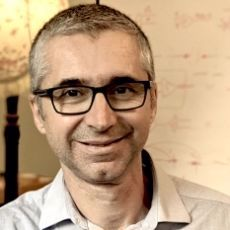
\includegraphics[width=0.25\textwidth]{imgs/ghica}
    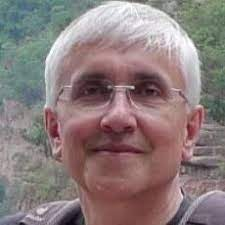
\includegraphics[width=0.25\textwidth]{imgs/achim}
    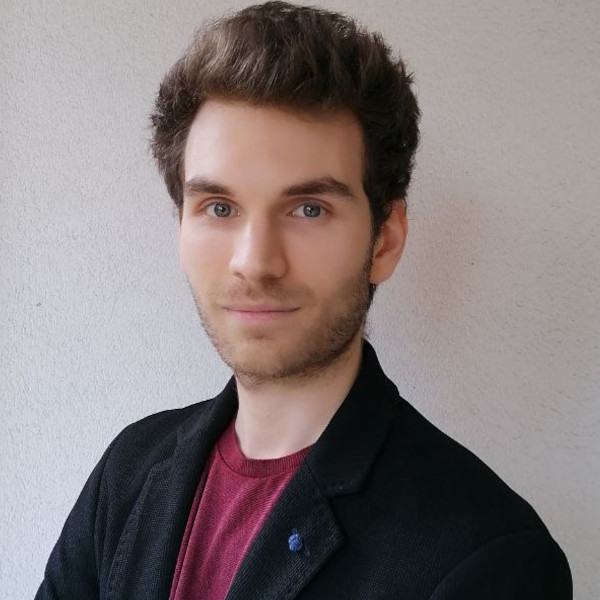
\includegraphics[width=0.25\textwidth]{imgs/lopez}

    \LARGE
    \textbf{Dan Ghica, Achim Jung, Aliaume Lopez}

    \normalsize
    \emph{`Diagrammatic semantics for digital circuits'}


\end{frame}

\begin{frame}
    \frametitle{The story so far}
    \vspace{0.5em}

    \centering

    \pause

    \begin{minipage}{0.49\textwidth}
        \centering
        \only<2>{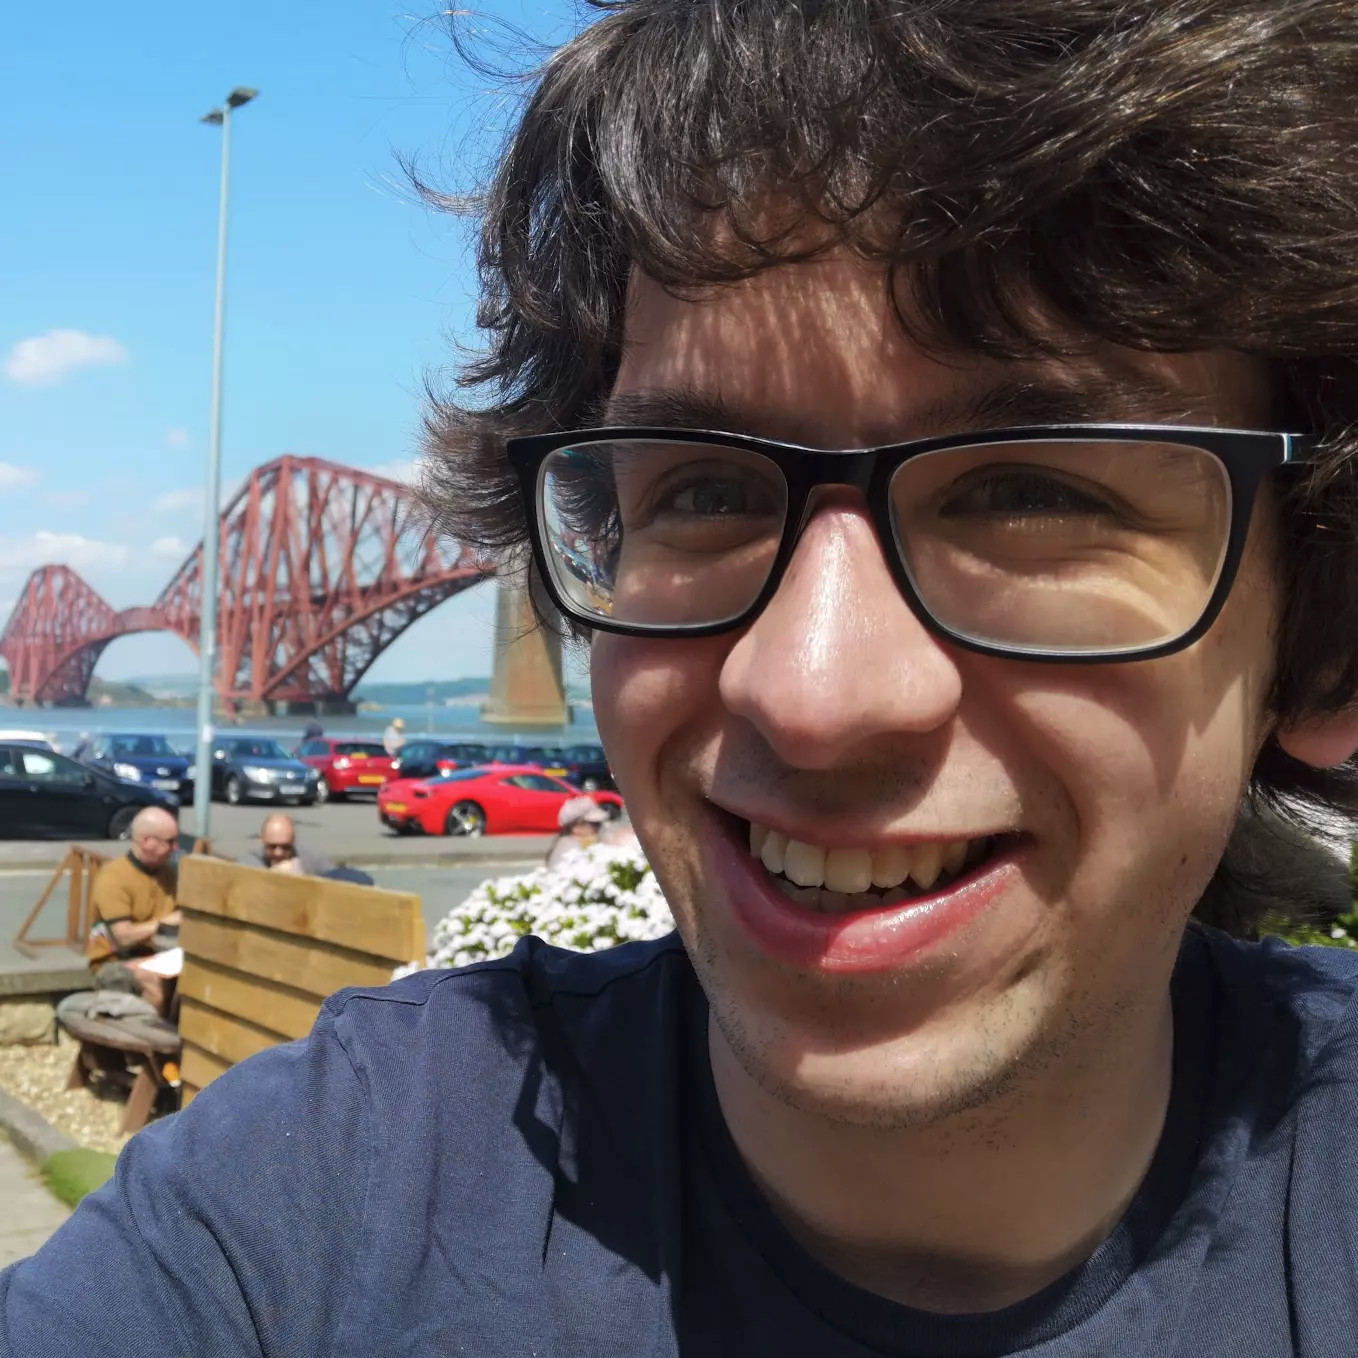
\includegraphics[width=0.5\textwidth]{imgs/kaye}}
        \only<3->{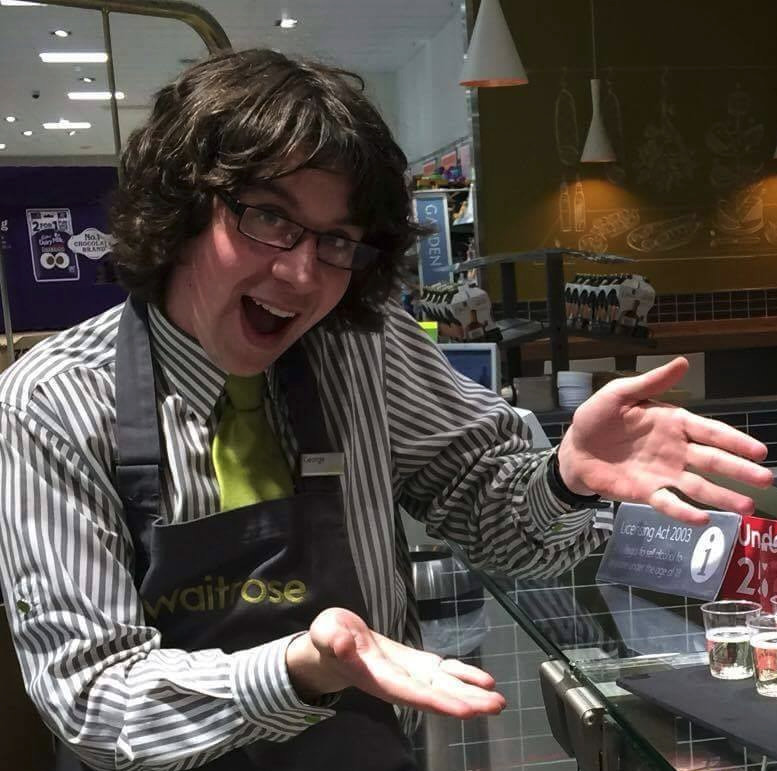
\includegraphics[width=0.5\textwidth]{imgs/kaye-waitrose}}

        \only<1->{\visible<6->{\emph{`Wow, this guy seems pretty groovy'}}}
    \end{minipage}
    \begin{minipage}{0.49\textwidth}
        \centering
        \only<2-4>{\visible<4>{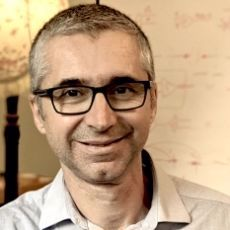
\includegraphics[width=0.5\textwidth]{imgs/ghica}}}
        \only<5->{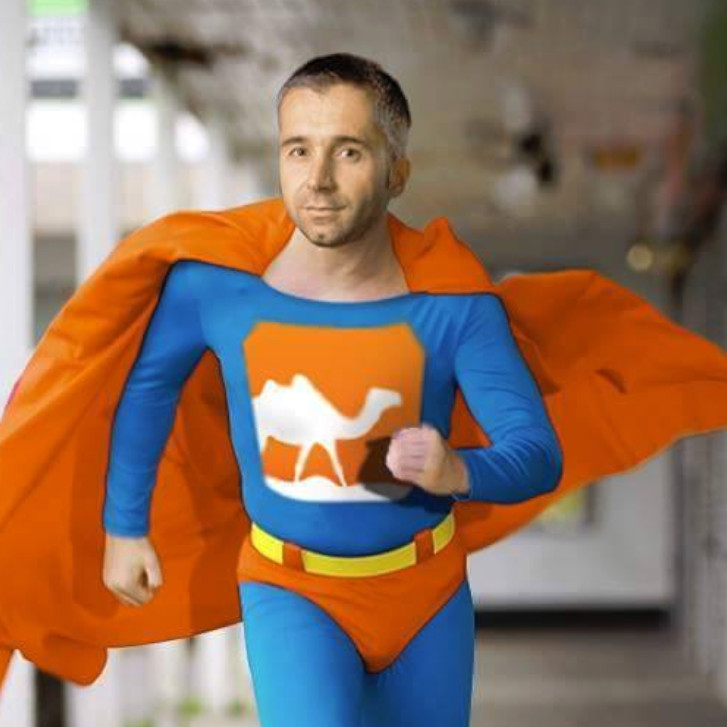
\includegraphics[width=0.5\textwidth]{imgs/ghica-ocaml}}

        \only<2->{\visible<7>{\emph{*OCaml noises*}}}
    \end{minipage}
\end{frame}

\begin{frame}
    \frametitle{The story so far}

    \centering

    \scalebox{8}{\textbf{2019}}

\end{frame}

\begin{frame}
    \frametitle{The story so far}

    \centering

    \begin{minipage}{0.49\textwidth}
        \centering
        \only<1>{
\includegraphics[width=0.5\textwidth]{imgs/kaye-grad}}
        \only<2->{
\includegraphics[width=0.5\textwidth]{imgs/kaye-phd}}

        \visible<5->{\emph{`No'}}

        \visible<7->{\emph{`Okay'}}
    \end{minipage}
    \begin{minipage}{0.49\textwidth}
        \centering
        \visible<3->{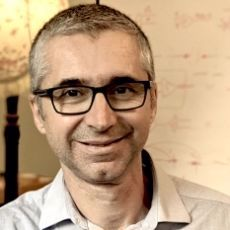
\includegraphics[width=0.5\textwidth]{imgs/ghica}}

        \visible<4->{\emph{`Do you know category theory'}}

        \visible<6->{\emph{`Do you want to do circuits stuff'}}
    \end{minipage}
\end{frame}

\begin{frame}
    \frametitle{The story so far}

    \centering

    \scalebox{8}{\textbf{2021}}

\end{frame}

\begin{frame}
    \frametitle{The story so far}

    \centering

    \vspace{1em}

    \(
        \visible<2->{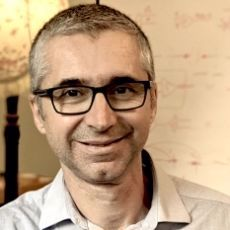
\includegraphics[width=0.2\textwidth]{imgs/ghica}}
        \visible<3->{\raisebox{3em}{ \(+\) }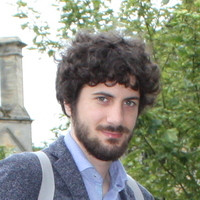
\includegraphics[width=0.2\textwidth]{imgs/zanasi}}
        \visible<4->{\raisebox{3em}{ \(=\) } 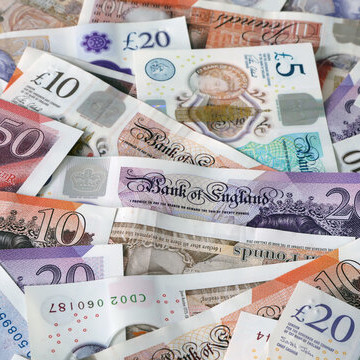
\includegraphics[width=0.2\textwidth]{imgs/money}}
    \)

    \vspace{1em}

    \(
        \visible<5->{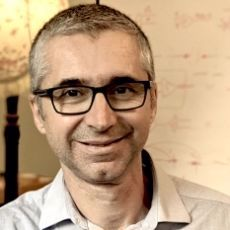
\includegraphics[width=0.2\textwidth]{imgs/ghica}}
        \visible<6->{\raisebox{3em}{ \(+\) }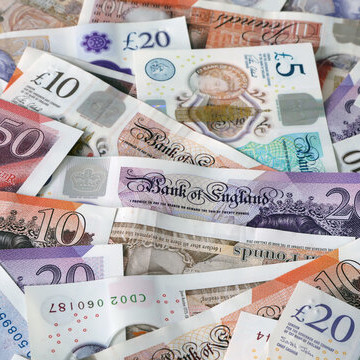
\includegraphics[width=0.2\textwidth]{imgs/money}}
        \visible<7->{\raisebox{3em}{ \(=\) } 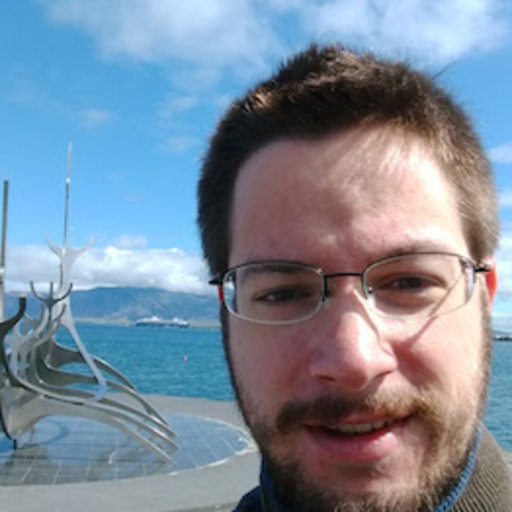
\includegraphics[width=0.2\textwidth]{imgs/sprunger}}
    \)


\end{frame}

\begin{frame}
    \frametitle{The story so far}

    \centering

    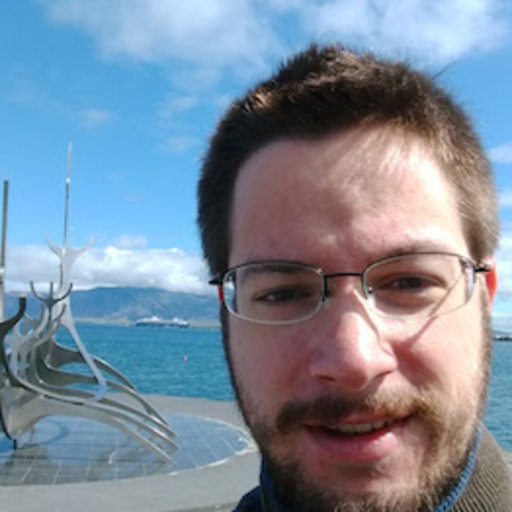
\includegraphics[width=0.25\textwidth]{imgs/sprunger}

    \LARGE
    \textbf{David Sprunger}

    \pause
    \normalsize
    (now at Indiana State University)

\end{frame}

\begin{frame}
    \frametitle{Let's get dangerous}

    \centering

    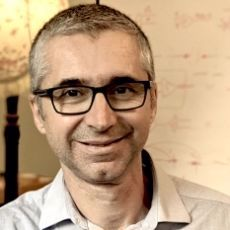
\includegraphics[width=0.25\textwidth]{imgs/ghica}
    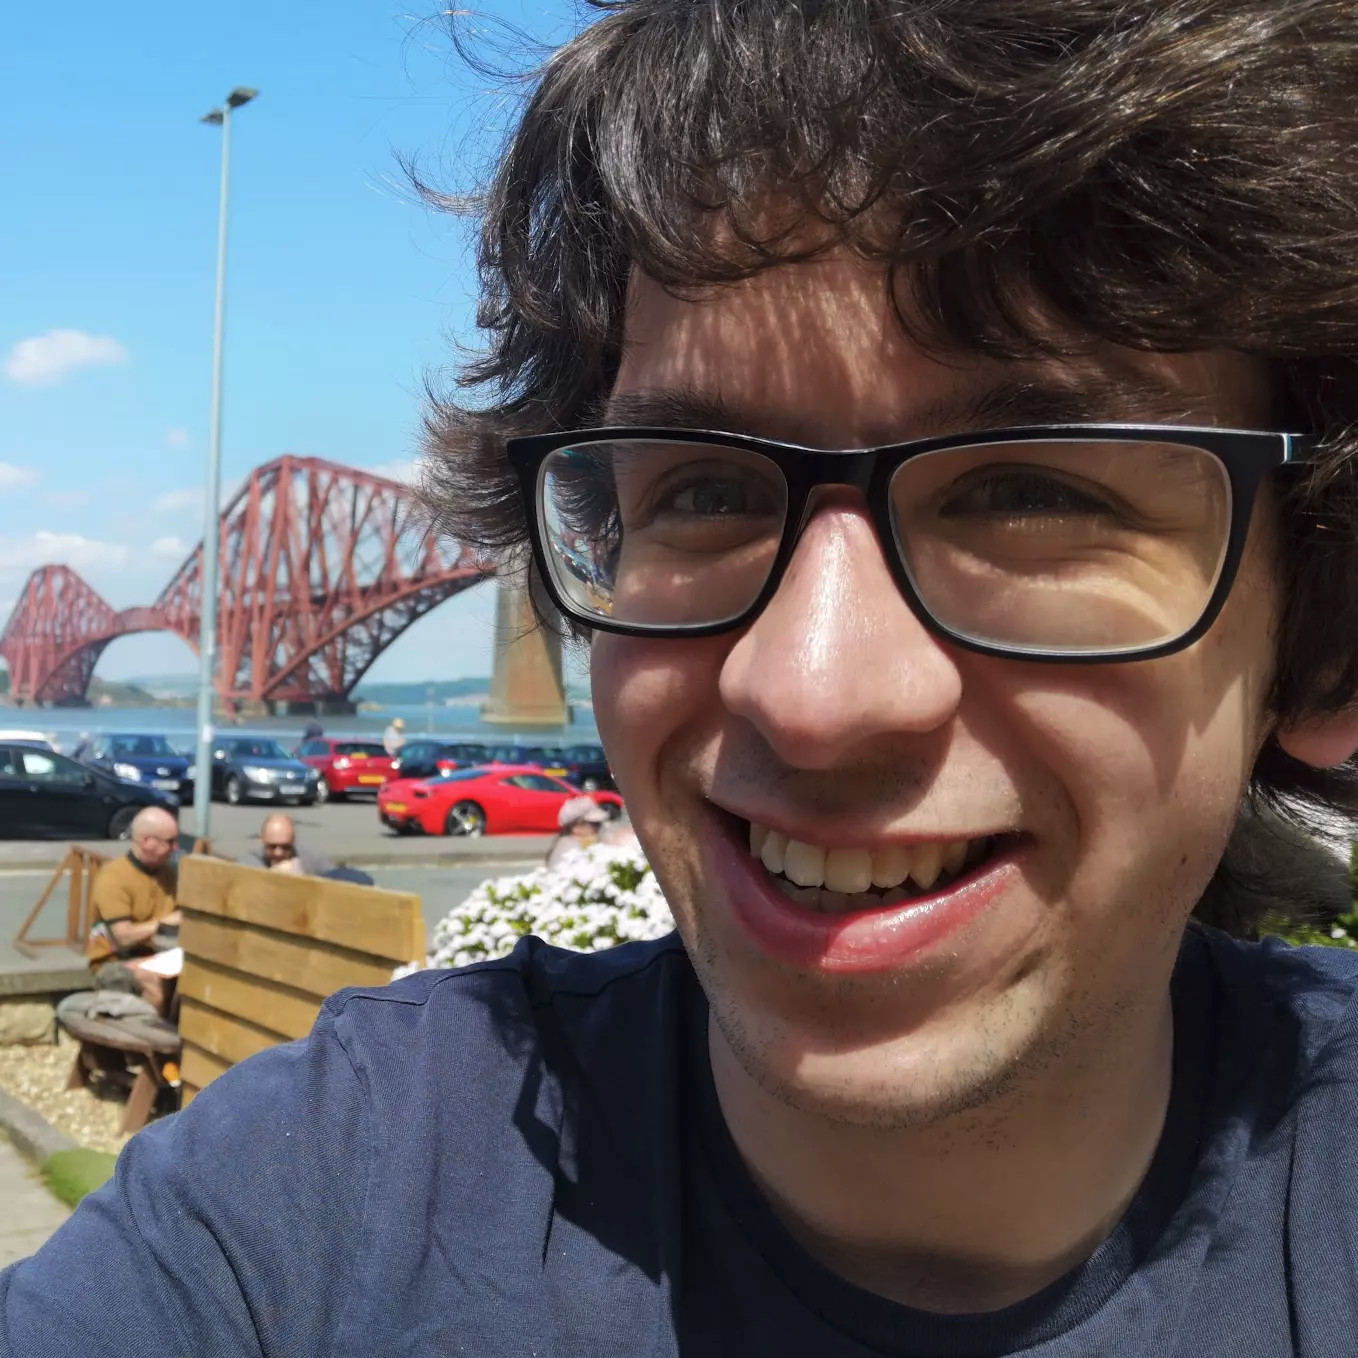
\includegraphics[width=0.25\textwidth]{imgs/kaye}
    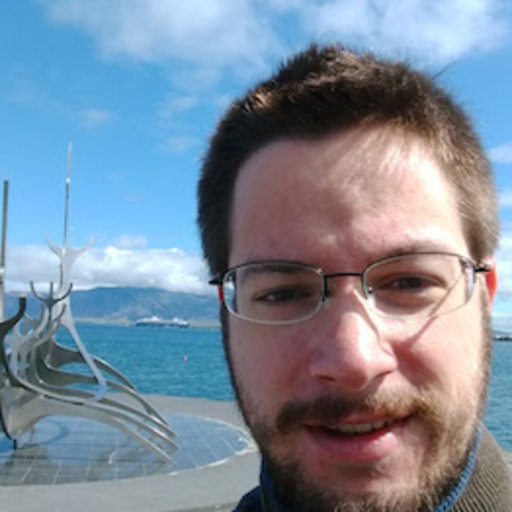
\includegraphics[width=0.25\textwidth]{imgs/sprunger}

\end{frame}